\bookchapter{UDP Networking}\label{ch:rust7}

\section*{Explanation}
The robot and the debug client talk over the network, and the protocol of our team is built on \textbf{UDP}. This chapter shows how to send and receive UDP packets in Rust, how to design a small binary packet, how to make a receiver that survives lost, repeated and broken packets, and how to measure what the network does. Networks and sockets in general were the topic of Chapters~\ref{ch:hw2} and~\ref{ch:linux7}; here we use them from a program. Only the standard library is needed (\verb!std::net!), and all programs of this chapter were compiled and run (on the loopback interface of one computer; the behaviour between two computers can differ, see below).

\section*{UDP in a minute}
\begin{center}
\begin{tikzpicture}[>={Stealth[length=2.4mm]},font=\footnotesize]
 \node[font=\bfseries\footnotesize] at (1.5,3.1) {TCP};
 \node[font=\bfseries\footnotesize] at (8.5,3.1) {UDP};
 \draw[thick] (0.2,0) -- (0.2,2.8); \draw[thick] (2.8,0) -- (2.8,2.8);
 \draw[->] (0.2,2.5)--(2.8,2.3); \draw[<-] (0.2,2.2)--(2.8,2.0); \node[font=\scriptsize] at (1.5,2.7) {connect};
 \draw[->,thick] (0.2,1.6)--(2.8,1.4); \draw[<-,dashed] (0.2,1.3)--(2.8,1.1); \node[font=\scriptsize] at (1.5,1.75) {data, acknowledged};
 \node[font=\scriptsize,align=center] at (1.5,0.5) {a reliable stream;\\ lost data is resent\\ (and everything waits)};
 \draw[thick] (7.2,0) -- (7.2,2.8); \draw[thick] (9.8,0) -- (9.8,2.8);
 \draw[->,thick] (7.2,2.4)--(9.8,2.25); \draw[->,thick] (7.2,1.9)--(9.8,1.75);
 \draw[->,thick] (7.2,1.4)--(8.4,1.33); \node[red] at (8.6,1.30) {$\times$};
 \draw[->,thick] (7.2,0.95)--(9.8,0.82);
 \node[font=\scriptsize,align=center] at (8.5,0.2) {separate messages (datagrams);\\ no connection, no resend};
\end{tikzpicture}
\captionof{figure}{TCP delivers a stream and waits for lost data; UDP delivers single messages and lets some be lost.}
\end{center}
A \textbf{UDP datagram} is one message with a source and a destination address (an IP address plus a port number). Compared with TCP:
\begin{itemize}[nosep]
\item no connection set-up, a message can be sent at any time to anybody;
\item packets can be \textbf{lost}, \textbf{duplicated}, or arrive in a \textbf{different order}; the program must cope with it;
\item the boundaries of a message are preserved (one \verb!send! gives one \verb!recv!), unlike a TCP stream;
\item a message is limited in size: an Ethernet frame carries at most $1500$ bytes (the \textbf{MTU}); after $20$ bytes of IPv4 header and $8$ bytes of UDP header, a payload of $1472$ bytes fits into one frame. Bigger datagrams are \emph{fragmented} and are lost completely if one fragment is lost. Keep messages below about $1400$ bytes;
\item no waiting for resent data: a late sensor value is replaced by the next one, which is exactly what a robot wants. This is also why ROS~2 and DDS use UDP for sensor data (Chapter~\ref{ch:ros2}).
\end{itemize}
TCP is the right choice when every byte must arrive (files, commands that must not be lost); we use UDP for streams of values where the \emph{newest} matters.

\section*{Sending and receiving}
%rs:echo
\begin{verbatim}
use std::net::UdpSocket;
use std::thread;

fn main() -> std::io::Result<()> {
    let server = UdpSocket::bind("127.0.0.1:0")?;   // port 0: OS picks one
    let addr = server.local_addr()?;
    let t = thread::spawn(move || -> std::io::Result<()> {
        let mut buf = [0u8; 1500];
        let (n, from) = server.recv_from(&mut buf)?;  // waits for a packet
        server.send_to(&buf[..n], from)?;             // echo it back
        Ok(())
    });

    let client = UdpSocket::bind("127.0.0.1:0")?;
    client.send_to(b"ping", addr)?;
    let mut buf = [0u8; 1500];
    let (n, _from) = client.recv_from(&mut buf)?;
    println!("got {n} bytes: {:?}", &buf[..n]);
    println!("as text: {}", String::from_utf8_lossy(&buf[..n]));
    t.join().unwrap()?;
    Ok(())
}
\end{verbatim}
prints
\begin{verbatim}
got 4 bytes: [112, 105, 110, 103]
as text: ping
\end{verbatim}
The most important calls:
\begin{center}
\renewcommand{\arraystretch}{1.2}
\begin{tabular}{lp{8.5cm}}
\verb!UdpSocket::bind(addr)! & open a socket on a local address and port; \verb!"0.0.0.0:9000"! means ``all interfaces'', \verb!"127.0.0.1:..."! only this computer\\
\verb!send_to(&bytes, addr)! & send one datagram; returns the number of bytes sent\\
\verb!recv_from(&mut buf)! & wait for a datagram, returns \verb!(length, sender)!; if the buffer is smaller than the packet, the rest is thrown away\\
\verb!connect(addr)! & remember a peer; then \verb!send!/\verb!recv! can be used and packets from others are ignored\\
\verb!set_read_timeout(Some(d))! & \verb!recv! returns an error after \verb!d! instead of waiting for ever\\
\verb!set_nonblocking(true)! & \verb!recv! returns at once with \verb!WouldBlock! if nothing is there\\
\verb!set_broadcast(true)! & allow sending to a broadcast address, for discovery\\
\end{tabular}
\end{center}
Everything returns an \verb!io::Result!, because a network can always fail (Chapter~\ref{ch:rust5}); the operator \verb!?! passes the error on. A buffer is an array of bytes \verb![u8; N]! on the stack. \verb!&buf[..n]! is the part that was filled, a slice (Chapter~\ref{ch:rust3}); \verb!b"ping"! is a byte string, an array of bytes written like a text.

\section*{A binary packet}
Text formats like JSON are easy to read but big and slow to parse. For a robot that sends sensor data $100$ times per second, a fixed binary layout is smaller and trivial to decode. (Chapter~\ref{ch:rust8} shows protobuf, which gives a compact format \emph{and} lets the format grow; here we build a packet by hand, to understand what a serialization library does for you.) Our packet has $28$ bytes:
\begin{center}
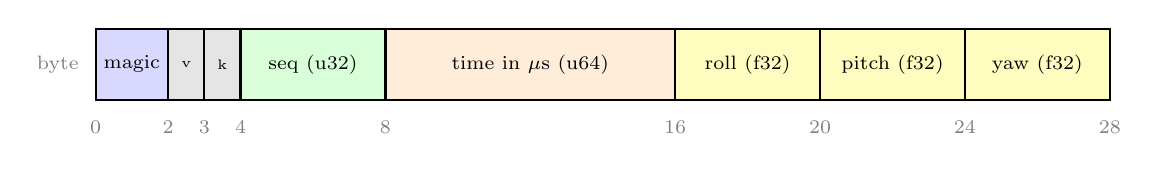
\begin{tikzpicture}[font=\scriptsize,x=0.46cm]
 \foreach \a/\b/\t/\c in {0/2/magic/blue!15, 2/3/{\tiny v}/gray!20, 3/4/{\tiny k}/gray!20, 4/8/seq (u32)/green!15, 8/16/time in $\mu$s (u64)/orange!15, 16/20/roll (f32)/yellow!25, 20/24/pitch (f32)/yellow!25, 24/28/yaw (f32)/yellow!25}{
   \draw[fill=\c,thick] (\a,0) rectangle (\b,0.9); \node[align=center] at ({(\a+\b)/2},0.45) {\t};}
 \foreach \p in {0,2,3,4,8,16,20,24,28} {\node[gray] at (\p,-0.35) {\p};}
 \node[gray,anchor=east] at (-0.2,0.45) {byte};
\end{tikzpicture}
\captionof{figure}{Layout of the example packet (v = version, k = kind). Every number has a fixed size and a fixed position.}
\end{center}
Multi-byte numbers can be stored with the least significant byte first (\textbf{little endian}: x86 and ARM processors) or last (\textbf{big endian}: the traditional ``network byte order''). The number $258=0x0102$ is the bytes \verb!02 01! in little endian and \verb!01 02! in big endian. Whatever you choose, \emph{both sides must agree}; Rust makes you say it: \verb!to_le_bytes()!, \verb!to_be_bytes()!, \verb!from_le_bytes()!, \verb!from_be_bytes()!. There is no way to forget it.
%rslib:packet
\begin{verbatim}
const MAGIC: u16 = 0xB07;
const LEN: usize = 28;

#[derive(Debug, Clone, PartialEq)]
pub struct Telemetry { pub seq: u32, pub t_us: u64, pub rpy: [f32; 3] }

#[derive(Debug, PartialEq)]
pub enum DecodeError { TooShort(usize), BadMagic(u16), BadVersion(u8) }

impl Telemetry {
    pub fn encode(&self) -> [u8; LEN] {
        let mut b = [0u8; LEN];
        b[0..2].copy_from_slice(&MAGIC.to_le_bytes());
        b[2] = 1;                                   // version
        b[3] = 0;                                   // kind: 0 = telemetry
        b[4..8].copy_from_slice(&self.seq.to_le_bytes());
        b[8..16].copy_from_slice(&self.t_us.to_le_bytes());
        for i in 0..3 {
            let at = 16 + 4 * i;
            b[at..at + 4].copy_from_slice(&self.rpy[i].to_le_bytes());
        }
        b
    }

    pub fn decode(b: &[u8]) -> Result<Telemetry, DecodeError> {
        if b.len() < LEN { return Err(DecodeError::TooShort(b.len())); }
        let magic = u16::from_le_bytes([b[0], b[1]]);
        if magic != MAGIC { return Err(DecodeError::BadMagic(magic)); }
        if b[2] != 1 { return Err(DecodeError::BadVersion(b[2])); }
        let f = |i: usize| {
            f32::from_le_bytes(b[i..i + 4].try_into().unwrap())
        };
        Ok(Telemetry {
            seq: u32::from_le_bytes(b[4..8].try_into().unwrap()),
            t_us: u64::from_le_bytes(b[8..16].try_into().unwrap()),
            rpy: [f(16), f(20), f(24)],
        })
    }
}

#[cfg(test)]
mod tests {
    use super::*;

    #[test]
    fn roundtrip() {
        let t = Telemetry {
            seq: 7, t_us: 123_456_789, rpy: [0.5, -1.25, 90.0],
        };
        let b = t.encode();
        println!("{:02x?}", &b[..8]);
        assert_eq!(Telemetry::decode(&b), Ok(t));
    }

    #[test]
    fn rejects_bad_input() {
        let e = Telemetry::decode(&[1, 2, 3]);
        assert_eq!(e, Err(DecodeError::TooShort(3)));
        let mut b = Telemetry { seq: 0, t_us: 0, rpy: [0.0; 3] }.encode();
        b[0] = 0;
        let e = Telemetry::decode(&b);
        assert!(matches!(e, Err(DecodeError::BadMagic(_))));
    }

    #[test]
    fn random_bytes_never_panic() {
        let mut x: u64 = 88172645463325252;      // xorshift random numbers
        let (mut ok, mut err) = (0, 0);
        for _ in 0..1_000_000 {
            let mut b = [0u8; 40];
            for byte in b.iter_mut() {
                x ^= x << 13; x ^= x >> 7; x ^= x << 17;
                *byte = x as u8;
            }
            let n = (x % 41) as usize;                 // length 0..=40
            match Telemetry::decode(&b[..n]) {
                Ok(_) => ok += 1,
                Err(_) => err += 1,
            }
        }
        println!("ok {ok}, err {err}");
        assert_eq!(ok + err, 1_000_000);
    }
}
\end{verbatim}
\verb!cargo test -- --nocapture! shows (the real run):
\begin{verbatim}
[07, 0b, 01, 00, 07, 00, 00, 00]
ok 0, err 1000000
\end{verbatim}
and three passed tests. The first eight bytes show the little-endian layout: \verb!07 0b! is the magic $0x0B07$, the version \verb!01!, the kind \verb!00!, then the sequence number $7$ in four bytes. The random-input test sent one million random buffers of random length to the decoder: it \emph{never panicked}, and none was accepted (the chance that two random bytes have the magic value is $1/65536$, and the length must be right as well; to see accepted packets one would have to mutate valid ones). This kind of test is cheap and catches the typical errors: missing length checks and out-of-range slices. A decoder that gets its data from a network \textbf{must never trust the packet}: check the length first, then the magic and the version, only then read the fields. (A real fuzzer such as \verb!cargo fuzz! does this much more cleverly.)

The decoder uses \verb!b[4..8].try_into().unwrap()!: converting a slice of length $4$ to an array \verb![u8; 4]! cannot fail \emph{after} the length check, so the \verb!unwrap! is justified, one of the rare cases (Chapter~\ref{ch:rust5}). If you have an \verb!f32! from a sensor it takes $4$ bytes: a ``field of $3$ floats'' is $12$ bytes, against the roughly $50$ characters of a JSON text with the same information.

\section*{Lost, duplicated, reordered}
Every packet carries a \textbf{sequence number}. The receiver compares it with the last one it has seen:
\begin{center}
\renewcommand{\arraystretch}{1.2}
\begin{tabular}{ll}
\textbf{new seq vs.\ last} & \textbf{meaning}\\ \hline
last $+1$ & normal\\
more than last $+1$ & packets lost: the gap is counted\\
equal to last, or smaller (a small step) & duplicate or late packet: ignore it\\
much smaller (e.g.\ $0$ after $50\,000$) & the sender has restarted: reset the counter\\
\end{tabular}
\end{center}
Use \verb!wrapping_sub! to compare, because the counter eventually overflows (Chapter~\ref{ch:rust2}). The following program sends $100$ packets over loopback, throws away every fourth one at the sender (to simulate a bad wireless link), and lets the receiver count the loss and compute statistics.
%rs:loss
\begin{verbatim}
use std::net::UdpSocket;
use std::time::Duration;

fn main() -> std::io::Result<()> {
    let rx = UdpSocket::bind("127.0.0.1:0")?;
    rx.set_read_timeout(Some(Duration::from_millis(200)))?;
    let tx = UdpSocket::bind("127.0.0.1:0")?;
    for seq in 0u32..100 {
        if seq % 4 == 3 { continue; }               // "lost on the way"
        tx.send_to(&seq.to_le_bytes(), rx.local_addr()?)?;
    }
    let (mut last, mut got, mut lost) = (None::<u32>, 0, 0);
    let mut buf = [0u8; 64];
    loop {
        let n = match rx.recv_from(&mut buf) {
            Ok((n, _)) => n,
            Err(e) if e.kind() == std::io::ErrorKind::WouldBlock
                   || e.kind() == std::io::ErrorKind::TimedOut => break,
            Err(e) => return Err(e),
        };
        if n < 4 { continue; }
        let seq = u32::from_le_bytes(buf[..4].try_into().unwrap());
        if let Some(l) = last {
            let step = seq.wrapping_sub(l);
            if step == 0 || step > u32::MAX / 2 { continue; }   // dup / old
            lost += step - 1;
        }
        last = Some(seq);
        got += 1;
    }
    println!("received {got}, lost {lost}");
    Ok(())
}
\end{verbatim}
prints \verb!received 75, lost 24!. The 25 dropped packets are numbers $3,7,\dots,99$; the last one, $99$, is dropped at the end, so the receiver cannot know about it: a loss at the end of a stream is invisible without a time-out or a heartbeat. This is why a UDP receiver also needs a clock: ``no packet for $200$\,ms'' is itself an event (the robot may have fallen over, the client may have closed), and the user interface should show it.

\section*{A receive loop for a robot}
The structure of a receiving thread that works well with Chapter~\ref{ch:rust6}:
\begin{verbatim}
fn rx_loop(sock: UdpSocket, out: Sender<Telemetry>, run: Arc<AtomicBool>) {
    sock.set_read_timeout(Some(Duration::from_millis(100))).unwrap();
    let mut buf = [0u8; 2048];                  // bigger than any message
    while run.load(Ordering::Relaxed) {
        match sock.recv_from(&mut buf) {
            Ok((n, _from)) => match Telemetry::decode(&buf[..n]) {
                Ok(t) => { let _ = out.send(t); }
                Err(_) => { /* count it, do not stop */ }
            },
            Err(e) if is_timeout(&e) => { /* no data: check the flag */ }
            Err(e) => { eprintln!("socket error: {e}"); break; }
        }
    }
}
\end{verbatim}
The read time-out is important: a thread blocked in \verb!recv_from! cannot see the stop flag; with a time-out it wakes up ten times a second and ends cleanly. Errors in the decoder are counted, not fatal. For a control loop that wants only the \emph{newest} packet (Chapter~\ref{ch:rust6}), read in the non-blocking mode until the socket is empty, and keep the last valid one.

\section*{How fast is the network? Measuring the round trip}
A ping-pong test with the echo server of the first example, $20\,000$ round trips of a $28$-byte packet on loopback, gave on the computer of this book (two runs, release build) a median round-trip time of $26$ to $30\,\mu$s and a $99$th percentile of about $60\,\mu$s, but a worst case of $330\,\mu$s in one run and $2.3$\,ms in the other (Chapter~\ref{ch:ai9} explains why one looks at percentiles and the maximum, not the mean). A loopback round trip involves two system calls per direction and the scheduler of the operating system, but no network card; a real Ethernet link adds about $100\,\mu$s for a cable, several milliseconds for Wi-Fi, with a very irregular \textbf{jitter}. For the robot, what matters is the \emph{worst} delay, not the average, which is why a control loop never waits for a packet.

\section*{Firewalls, addresses and broadcast}
Between two computers you must check three things that loopback hides: (1) the \textbf{address}: the server binds \verb!0.0.0.0:port! (all interfaces), the client sends to the IP address of the robot (\verb!ip a! shows it, Chapter~\ref{ch:linux7}); (2) the \textbf{firewall}: on Ubuntu \verb!sudo ufw status! and, if needed, \verb!sudo ufw allow 9000/udp!; (3) the \textbf{network}: Wi-Fi at a tournament often \emph{isolates clients} or blocks broadcast, in which case no program helps; ask the organisers, or use your own router. Tools for debugging: \verb!ss -ulpn! (which program listens on which UDP port), \verb!nc -u -l 9000! and \verb!nc -u robot 9000! (a quick sender and receiver), \verb!sudo tcpdump -i any -n udp port 9000! (see the packets). If you know the robot only by name, \verb!"robot.local:9000"! is resolved by the standard library when you pass a string to \verb!send_to!. Multicast and broadcast (sending to many receivers with one packet) work with \verb!set_broadcast(true)! and \verb!join_multicast_v4!; DDS uses multicast for discovery (Chapter~\ref{ch:ros2}). These calls exist in \verb!std::net! but were not run for this book, because the test computer has only a loopback network.

\begin{aibox}[Design rules for a robot UDP protocol]
(1) Every packet starts with a magic number, a version and a type. (2) Every packet has a sequence number and a time stamp. (3) Never trust the length or the content: decode defensively, count errors. (4) Keep a packet below $1400$ bytes. (5) Send a regular heartbeat so the other side can notice silence. (6) Commands that must not be lost get an acknowledgment and are resent, or go over TCP; streams of measurements do not. (7) Write the layout \emph{once}, in a shared library or in a protocol description file (Chapter~\ref{ch:rust8}), and generate both sides from it.
\end{aibox}

\section*{Practice problems}
\begin{enumerate}[label=\textbf{\thechapter.\arabic*}]
  \item Give two properties of UDP that a robot's sensor stream profits from and two that are a problem. How does a program solve each problem?
  \item What is the largest UDP payload that fits into one Ethernet frame (MTU $1500$)? What happens if you send $3000$ bytes? How many bytes does a packet with $22$ joint angles as \verb!f32! need, and how many a JSON text with $22$ numbers like \verb!"0.123456"!?
  \item Write down the bytes (hexadecimal) of the following numbers in little endian and in big endian: the \verb!u16! $0x1234$, the \verb!u32! $1$, the \verb!u32! $258$. Check with a Rust program using \verb!to_le_bytes! and \verb!to_be_bytes!.
  \item Write a program that binds a UDP socket on \verb!127.0.0.1:0!, sends itself the message \verb!"hello"! and prints what it receives and from which address.
  \item Extend the packet of the chapter with a field \verb!battery: f32! (new size: $32$ bytes). Which functions change? What should happen with the version number and with receivers that still understand only the old format?
  \item A receiver sees the sequence numbers $10,11,12,15,15,14,16$. For each number say what the code of this chapter does (count of lost packets, ignore, reset).
  \item Write a function \verb!fn drain_latest(sock: &UdpSocket) -> Option<Telemetry>! for a non-blocking socket that reads all waiting packets and returns the newest valid one. Why is this better for a control loop than reading one packet per cycle?
  \item The receiver shows ``connected'' as long as packets arrive. Describe how to detect that the sender has gone, which time-out you choose for a sender that sends $100$ packets per second, and why a time-out of exactly the packet period would be a bad choice.
  \item Your program works on the laptop with \verb!127.0.0.1! but not between the laptop and the robot. List four things you check, in a sensible order, with the command for each.
  \item[\textbf{\thechapter.10}$\star$] Write a program with a ``robot'' thread that sends a telemetry packet every $10$\,ms with the next sequence number, and a ``client'' thread that receives for $1$ second and prints the number of packets, the number of losses, and the median and maximum interval between packets (in ms). Run it in the release mode. What do you expect for the interval, and what might make the maximum much larger?
\end{enumerate}
